\setlength\parindent{0pt} 

\subsection{Wavenumber, angular frequency, complex plane} We know that for
a wave, $1 (\text{cycle}) = 2\pi (\text{rad}) = 1 (\lambda = x (m))$.  \begin{itemize} \item
wavenumber spatial frequency of a wave: \\ \begin{equation} k  = \frac{2 \pi \text{(rad)}}{\lambda
\text{(m)}} = \frac{1 \text{(cycle)}}{\lambda \text{(m)}} \end{equation} shows how many cycles per
unit distance or radians per unit distance a single wavelength ($\lambda$) has.  Its a measure of
spatial frequency (number of rads or cycles "per" meter), so the longer (shorter) wavelength occurs
less (more) frequent in a unit distance.  \item angular frequency of a wave: \\ \begin{equation}
\omega  = \frac{2 \pi \text{(rad)}}{T \text{(m)}} = \frac{1 \text{(cycle)}}{T \text{(m)}},
\end{equation} shows how many cycles or radians a wave has per second.  \item relationship to
complex plane: \\ The unit circle on the complex plane with $|z|=1$ is $z = e^{i(kx-\omega t)}$.
The units for $kx$ is "cycle", thus $k$ is a measure of rate of rotation in a circle as a wave
propagates.  \begin{exmp} For a wave of $k=0.1$, it needs to travel $2\pi/0.1= 62.8(m)$ (single
wavelength) for a full circle/cycle.  Whereas $k=10$ only requires $6.28(m)$ to travel a full
circle.  Therefore a wave rotates faster (shorter wavelength) in a complex circle as the $k$
increases.  \end{exmp} \item Visualizing a wave interacting with a complex plane: \\ Draw a three
dimensional cartesian coordinate with $x$ on one axis and the other two are the complex plane axes.
Draw a wave $f(x)=\cos(kx)$ running with a fixed $k$ to an arbitrary $x$.  The complex number can be
seen as a vector-valued function $z=g(x)=(\cos(kx),\sin(kx))$ mapping $x$ to the complex plane
coordinate.  Thus as the wave propagates along $x$, the $z$ will be spinning in a circle on the
complex plane.  The "graph" $(x,g(x))$ is seen as a spring swirling along/around the $x$ axis.  The
numbers of wave in a unit distance $x=1$ can be seen on the graph $f(0 \ge x \le 1)$.  \item
Visualizing the angular velocity vector (in a rotating reference plane): \\ A vector that is
perpendicular to the rotational circle on a physical plane.  Lets focus on three orthogonal vectors,
$v$ (cross radial velocity vector), $\omega$ (angular velocity vector), $r$ (radial vector).  The
three coordinates are related by $\omega = \frac{d\theta}{dt} = \frac{1}{r}\frac{dx}{dt} =
\frac{v}{r}$, .  Thus we see that with a constant angular velocity, the smaller $r$ gives higher
$v$.  For an arbitrary velocity vector $\vect{v} = \vect{\omega} \times \vect{r}$.  \end{itemize}

\subsection{Inertial and non-inertial reference frame} A rotating reference frame (frame that
accelerates w.r.t. an inertial frame) is a non-inertial reference frame.  The Navier-Stokes equation
of the absolute velocity (inertial frame) is composed of the rotational velocity (rotating frame)
plus the velocity contributed by the angular velocity \begin{equation}
\Big(\frac{du_{\text{inert}}}{dt}\Big)_{\text{inert}} =
\Big(\frac{du_{\text{rot}}}{dt}\Big)_{\text{rot}} + 2\Omega \times u_{\text{rot}}.  \end{equation}
\begin{exmp} Suppose a ball going straight from north to south along a longitude when viewed from a
fixed point in the outer space.  This ball will seem to curve right, with westward velocity, when
viewed on earth.  Thus adding back the eastward rotational velocity will cancel the westward
velocity and transform the velocity back to the inertial frame, which is a straight southward
velocity.  \end{exmp}

\subsection{Field, Eulerian, Lagrangian} \begin{itemize} \item Eulerian framework (reference frame
fixed in space): \\ Different particles with the QoI measured at the same local point with time.
This gives the "field" of QoI if all spatial points are measured/modeled.  \item Lagrangian
framework (reference frame moving in space): \\ A particle with the QoI is measured by following the
particle parametrized by the intial position.  The instantaeous position $\bf{x}$ becomes a QoI
instead of a fixed value as in the Eulerian view.  \item \end{itemize}



\subsection{streamline} \begin{derv*} A streamline can be mapped out by solving for the instantaeous
spatial points that matches \begin{equation} \td t = \frac{\td x}{u} = \frac{\td y}{v}.
\end{equation} This condition must be satisfied when following a streamline. When given $u(t_1)$,
$v(t_1)$ and $\Delta t=t_2-t_1$, find $(x_2, y_2)$ for the entire field, connect the dots of
$(x_2,y_2)$ with the closest $(x_1,y_1)$ in the field gives the streamline. The streamlines show the
instantaneos directional path of the flow field.  \end{derv*}



\subsection{Material derivative/Lagrangian derivative} The acceleration of a particle in the
Eulerian field could be derived from the first order Taylor expansion of $u$ by following a particle
from $(x,t)$ to $(x+\delta x,t+\delta t)$, \begin{equation} \begin{aligned} & u(x+\delta x, t+\delta
t) \approx u(x,t) + \delta x \cdot\nabla u + \delta t \frac{\partial u}{\partial t} \\ &
\lim_{\delta t \to 0}\frac{u(x+\delta x, t+\delta t) - u(x,t)}{\delta t} = \frac{\partial
u}{\partial t} + u \cdot \nabla u. \\ \end{aligned} \end{equation} Imagine a flow with cold water
upstream and warm downstream. The particle temperature is the scalar QoI. Therefore, the particle at
any instant is locally heated by the sun which changes the first term. The changes due to motion
(spatial derivative), particle flows from cold to warm with velocity $\bm{u}$, then it recieves the
temperature gradient advection from the second term.

\subsection{Volume material derivative} A 2D squared volume at the initial time \begin{equation}
\delta V = \delta x \delta y = (x_2-x_1)(y_2-y_1).  \end{equation} At the next time step
\begin{equation} \begin{aligned} \delta V' & = \delta x' \delta y'  \\ & = (x_2+u_2\delta t -
(x_1+u_1\delta t))(y_2+v_2\delta t - (y_1+v_1\delta t)) \\ & = (\delta x + \delta u \delta t)(\delta
y + \delta v \delta t) \\ & = \delta V + \delta x \delta v \delta t + \delta y \delta u \delta t +
\delta t^2 \delta u \delta v.  \end{aligned} \end{equation} After some algebra \begin{equation}
\frac{\Delta \delta V}{\Delta t} = \delta x \delta y (\frac{\partial u}{\partial x} + \frac{\partial
v}{\partial y}) + \delta t \delta u \delta v.  \end{equation} The last term goes to zero as $\delta
t \rightarrow 0$, \begin{equation} \label{eq:volume} \frac{D \delta V}{D t} = \delta V \nabla \cdot
\vec{u}.  \end{equation}

\subsection{Gauss' Theorem (divergence theorem)} \begin{defn*} \begin{equation} \int \nabla \cdot Q
\td V = \int dA \cdot Q, \end{equation} which relates volume integral to a surface integral of a
scalar, vector or tensor field $Q$ (see \cite{chapin2010vector}, p155 for proof). Intuitively, the
sum of all sources minus the sinks in the volume equals the net flow going outward.  \end{defn*}



\subsection{linear strain rate} \begin{defn*} The rate of change of volume per unit volume
(expansion or contraction) \end{defn*} \begin{derv*} The rate of change per unit distance in
direction $x$ is (see Fig \ref{fig:linearStrain}) \begin{equation} \begin{aligned} \frac{1}{\delta
x} \frac{D \delta x}{D t} & = \frac{1}{\delta x} \frac{D}{D t} \big((u + \frac{\partial u}{\partial
x} \delta x) \delta t \big) - u \delta t \big)\\ & = \frac{\partial u}{\partial x} .  \end{aligned}
\end{equation} Therefore the rate of change in volume \begin{equation} \begin{aligned}
\frac{1}{\delta V} \frac{D \delta V}{D t} & = \frac{1}{\delta V} \frac{D \delta x \delta y \delta
z}{D t} \\ & = \frac{1}{\delta x} \frac{D \delta x}{D t} + \frac{1}{\delta y} \frac{D \delta y}{D t}
+ \frac{1}{\delta z} \frac{D \delta z}{D t} \\ & = \frac{\partial u}{\partial x} + \frac{\partial
v}{\partial y} + \frac{\partial w}{\partial z} \\ & = \frac{\partial u_i}{\partial x_i}
\end{aligned} \end{equation}

\end{derv*} 
\begin{figure}[H] 
   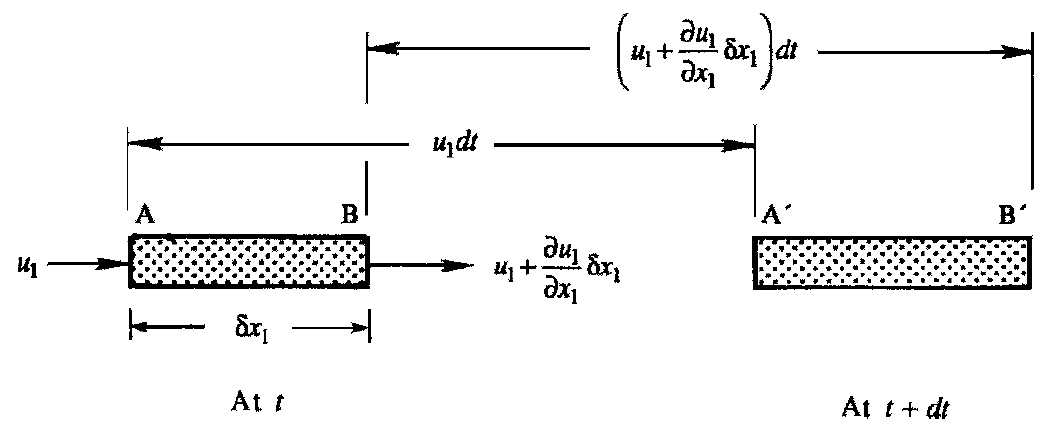
\includegraphics[width=0.7\textwidth,height=0.3\textwidth]{linearStrain.png} 
   \caption{\label{fig:linearStrain} From \cite{kundu2008fluid}.  } 
\end{figure}

\subsection{shear strain rate} 
\begin{defn*} 
The rate of decrease in angles of ``two" perpendicular lines (change in shape caused by squeezing,
and no change in volume) (see Fig \ref{fig:shearStrain}). For a single angle $\alpha$, 
\begin{equation} 
\begin{aligned} 
   \frac{\td \alpha }{\td t} 
   & = \frac{1}{\delta x_2}\frac{\td x_2}{\td t} \\ 
   & = \frac{1}{\delta x_2}\frac{((u_1 + \frac{\partial u_1}{\partial x_2}\delta x_2)\delta t - u_1
       \delta t ) }{\delta t} \\ 
   & = \frac{1}{\delta x_2}\frac{\td}{\td t}\big( \frac{\partial u_1}{\partial x_2}\delta x_2\delta t
       \big) \\ 
   & = \frac{\partial u_1}{\partial x_2} 
\end{aligned} 
\end{equation} 
(notice the small angle $\delta \theta = \frac{\delta x}{r}$, where $r$ is the radius and $\delta x$
is the arc length from C to A). Thus the total squeezing 
\begin{equation} 
  \frac{\td \alpha + \td \beta}{\td t} =
  \frac{\partial u_1}{\partial x_2} + \frac{\partial u_2}{\partial x_1} 
\end{equation} 
\end{defn*}
\begin{figure}[H] 
   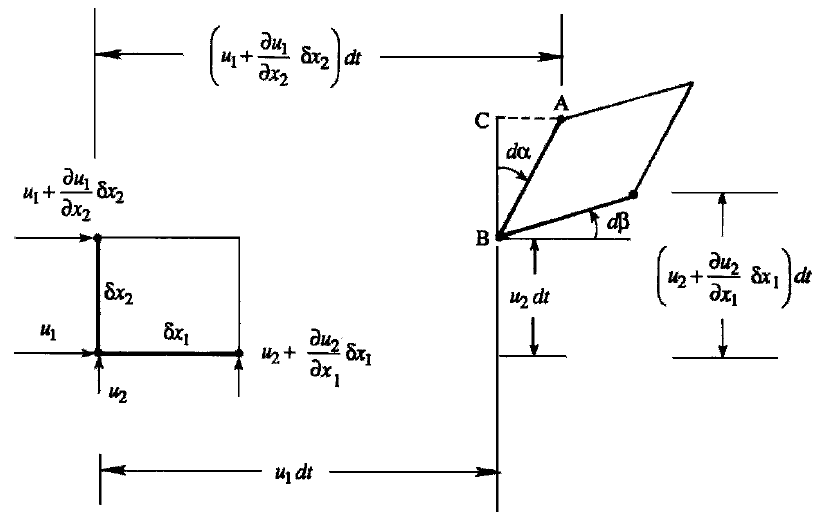
\includegraphics[width=0.6\textwidth, height=0.4\textwidth]{shearStrain.png}
   \caption{\label{fig:shearStrain} From \cite{kundu2008fluid}.  } 
\end{figure}

\subsection{strain rate tensor} 
\begin{defn*} 
The strain rate tensor (combining the linear and shear strain rate) 
\begin{equation} 
   e_{ij} = \frac{1}{2}(\frac{\partial u_i}{\partial x_j }+\frac{\partial u_j}{\partial x_i }) 
\end{equation} 
where the off-diagonal terms of $e_{ij}$ is half the shear strain rate. This tensor describes how a
fluid element deforms.  
\end{defn*}


\subsection{Mass continuity via material derivative} By definition, mass is conserved following a
particle, 
%
\begin{equation} 
\begin{aligned} 
   & \frac{D}{Dt} (\rho \delta V) = 0  \\ 
   & (\frac{D\rho}{Dt} + \rho\nabla \cdot \vect{v})\delta V = 0 \\ 
   & \int(\frac{D\rho}{Dt} + \rho\nabla\cdot\vect{v})dV = 0 \\ 
   & \int(\frac{\partial\rho}{\partial t} + \nabla\cdot(\rho\vect{v}))dV = 0 \\ 
\end{aligned} 
\end{equation} 
%
Applied \eqref{eq:volume} to the second line.  Applying divergence theorem to the last line gives 
%
\begin{equation}
   \int_V(\frac{\partial\rho}{\partial t})dV = -\int_V(\nabla\cdot(\rho\vect{v}))dV = -\int_S \vect{v}
\cdot d\vect{S} 
\end{equation} 
%
indicates the increase rate of density inside a particle equals the inflow rate from the surface of
the particle.


\subsection{Tangential Vector of a functional surface} 
The tangential vector at a point $x$ relative to the point at $y$ is $(y-x,f(y)-f(x))$, where the
first order Taylor expansion of $f(y) = f(x) + \nabla f(x)^T(y-x)$, which gives $(y-x,\nabla
f(x)^T(y-x))$.  


\subsection{Tensor} 
\subsubsection{Properties} 
Tensor, $T$, can be seen as a ``{\bf multilinear function}'' that eats in vectors and spits out a
scalar number, or a ``{\bf linear operator}'' that transforms vectors into vectors.  Multilinear $f
: V_1 \times \cdots \times V_n \rightarrow W$, means linear in each vector space (closed under
additivity and scalar multiplication). \\ 

\begin{exmp*} Moment of Inertia tensor ${\bf I}$ \\
By definition, moment of inertia is the angular momentum per unit angle per unit time.
\emph{ 
%
\begin{equation} 
   \text{KE} = \frac{1}{2} (\omega_x, \ \omega_y, \ \omega_z) 
   \begin{pmatrix} I_{xx} & I_{xy} & I_{xz} \\ I_{yx} & I_{yy} & I_{yz} \\ I_{zx} & I_{zy} & I_{zz} \\ 
   \end{pmatrix} 
   \begin{pmatrix} \omega_x \\ \omega_y \\ \omega_z 
   \end{pmatrix} 
\end{equation} 
%
where 
%
\begin{equation} L =   
   \begin{pmatrix} 
      I_{xx} & I_{xy} & I_{xz} \\ 
      I_{yx} & I_{yy} & I_{yz} \\ 
      I_{zx} & I_{zy} & I_{zz} \\ 
   \end{pmatrix} 
   \begin{pmatrix} 
      \omega_x \\
      \omega_y \\ 
      \omega_z.  
   \end{pmatrix} 
\end{equation} 
%
The first equation, $I$ is seen as a multilinear function that eats in two vectors of $\omega$ and
spits out a number $2$KE, $I(\omega,\omega) = 2\text{KE}$. The second equation, $I$ is seen as a
linear operator that eats in $\omega$ vector and spits out $L$ vector, $I(\omega) = L$. 
}
\end{exmp*}


\subsubsection{Components} 
A component of $T$ is just a value of the function $T$ on the given basis vectors, e.g. $T_{xx}=
T(\hat{x},\hat{x})$. 


\subsubsection{Multilinearity} 
Closed under addtivity and scalar multiplication on the separate vector spaces. \\ 
\begin{exmp*} 
rank 2 tensor 
\emph{ 
$T: V \times W \Rightarrow \mathcal{R}$.  $T$ is a rank $2$ multilinear function on $v$ and $w$ with
basis vectors $\hat{x}_1, \hat{x}_2$ if
\begin{equation*} 
\begin{aligned} 
   T(v,w) 
   & = T(v_1\hat{x}_1+v_2\hat{x}_2,w_1\hat{x}_1+w_2\hat{x}_2) \\ 
   & = v_1w_1T(\hat{x}_1,\hat{x}_1)+ v_1w_2T(\hat{x}_1,\hat{x}_2)+ v_2w_1T(\hat{x}_2,\hat{x}_1)+
       v_2w_2T(\hat{x}_2,\hat{x}_2) \\ 
   & = v_iw_jT_{ij}.  
\end{aligned} 
\end{equation*} 
}
\end{exmp*}

%It is a geometric object (like the box for stress tensor) that describe linear relations (dot
%product, cross product, linear maps) between vectors, scalars and other tensors.  It can be
%multi-dimensional array (e.g., 3D array or more).

%{\bf Examples} \\ Velocity gradient tensor $\frac{du_i}{dx_j}$, where the scalar $u_i$ (or the
%vector $u$) is operated by the vector $\nabla$.

%Advective tensor $u_j\frac{du_i}{dx_j}= (\bm u \cdot \nabla \bm u)_i$

\subsubsection{Covariant and Contravariant components of a vectors} In Cartesian coordinates, the
Length of vector $A$, $L_A= A_1^2+A_2^2$ and the dot-product of $A$ and $B$, $A \cdot B= A_1B_1 +
A_2B_2$. In non-Cartesian coordinates, the Length of the vector $A$, $L_A$ and $A\cdot B$ doesn't
work, which is why we need covariant and contravariant components. \\ Covariant components for $A$
is $(A_1,A_2)$ and Contravariant is $(A^1,A^2)$.  $L_A= A_1A^1+A_2A^2$.  The Covariant and
Contravariant is defined so that $L_A$ and $A\cdot B$ is unchanged.

Original definition of convariant and contravariant: \\ Given two basis, $e$ and $f$, for any
Euclidean vector $v= A e= B f$, $A=(a_1,\dotsc,a_n)^T, B=(b_1,\dotsc,b_n)^T$. Suppose the
transformation matrix, $T$, from $e$ to $f$ satisfies $f= Te$.  Therefore, $v= B T e$, thus $B T=
A$, which shows that $B= A T^{-1}$. In conclusion, the basis vector $e$ that is transformed covaries
with $f$, hence $e$ is transformed covariantly to a new basis $f$, and the components $A$ is
transformed contravariantly to the new basis $f$, with respect to the transformation $T$  \\
Covariant transformation: $A e=  BTe= Bf$. \\ Contravariant transformation: $A e= AT^{-1} f= Bf$. \\
\subsection{Upscale KE backscatter}

The $2$D Vorticity equation by streamfunction $\psi$

\begin{equation} \frac{D \nabla^2\psi}{D t} = F.  \end{equation}

Suppose there is no $F$, then by multiplying $-\psi$ and integrating over a domain A

\begin{equation} \begin{aligned} & \int_A \left( -\psi \frac{D\nabla^2\psi}{Dt} \right) dA= 0 \\ & =
\int_A \left( -\psi \nabla\frac{D\nabla\psi}{Dt} \right) dA \\ & = \int_A \left( -\cancel{\nabla
\left( \psi \frac{D \nabla\psi}{Dt} \right)} + \nabla \psi \frac{D\nabla\psi}{Dt} \right) dA \\ & =
\int_A \left( \frac{1}{2} \frac{D(\nabla\psi)^2}{Dt} \right) dA \\ & = \frac{D}{Dt} \int_A
\frac{1}{2} (\nabla\psi)^2 dA, \end{aligned} \end{equation}

which gives the domain integrated kinetic energy $E = \int_A\frac{1}{2} (\nabla\psi)^2 dA$ by using
periodic boundary condition or $v \cdot n= 0$, and $\frac{D E}{Dt}=0$.  Any function of the
vorticity is conserved after integrating over the domain A, $\frac{D}{Dt} \int_A g(\xi) dA= 0$.
Therefore 

\begin{equation} \begin{aligned} & \int_A -\frac{D}{Dt} (\psi \nabla^2\psi) dA= 0= \int_A \left(
-\psi \frac{D\nabla^2\psi}{Dt} \right) dA \\ & \frac{D}{Dt} \int_A -(\psi \nabla^2\psi) dA=
\frac{D}{Dt} \int_A \frac{1}{2} (\nabla\psi)^2 dA, \end{aligned} \end{equation}

where $E= -\int_A (\psi \nabla^2\psi) dA$.



\subsection{static pressure gradient force} Given surface depth $Z_1(x,y)$, and the second layer
surface $Z_2(x,y)$.  Pressure at a constant depth $z$ in layer $1$ equals $p_1= \rho g (Z_1- z)$.
Pressure at a constant depth $z$ in layer $2$ equals $p_2= \rho g Z_1 + \rho g' (Z_2- z)$.
Therefore, the horizontal pressure gradient at layer $1$ is $\nabla p_1= \rho g Z_1$ where the
constant depth $z$ is eliminated. Likewise, layer $2$ is $\nabla p_2= \nabla p_1 + \rho g' Z_2$. \\

{\bf Remarks}: This suggests the pressure gradient in each layer is just a function of the varying
surface height.


\subsection{Flux} \begin{defn*} rate of flow of a property (with some unit $U$) per unit area
($U m^{-2}s^{-1}$). \end{defn*}

\subsection{anelastic approximation} \begin{defn*} Suppose $\rho = \rho_0(z) + \rho^*(x,y,z,t)$
and $\rho \approx \rho_0$. From hydrostasy ($\frac{1}{\rho_0}\frac{\partial \bar{p}}{\partial z} - g
= 0$), the vertical equation of motion becomes \begin{equation} \frac{Dw}{Dt} = - \frac{1}{\rho_0}
\frac{\partial p^*}{\partial z} - g\frac{\rho^*}{\rho_0} + F.  \end{equation} Assume density doesn't
flutuate too fast with time ($\frac{D\rho}{Dt}=0$), then the mass continuity equation becomes
\begin{equation} \nabla \cdot \rho_0 v = 0.  \end{equation} \end{defn*}

\subsection{Boussinesq approximation} \begin{defn*} Same as anelastic approximation but assuming
shallow layer ($\rho_0 = $ constant), thus \begin{equation} \nabla \cdot v = 0.  \end{equation} This
allows a flux form substitution of the advection term for any variable. \end{defn*}


\subsection{dynamic viscosity} 
\begin{defn*} 
$\mu \big[ N s m^{-2}\big]$, the ``required" tangential force per unit area to move a parallel plane
at unit speed relative to a fixed plane at unit distance apart ($\mu = \tau/(\frac{\partial
u}{\partial z})$ = $\tau$ per unit speed per unit distance = standardized $\tau$). A bigger dynamic
viscosity  means more force is required to move
the two planes, thus more viscous.
\end{defn*}

\subsection{kinematic viscosity}
\begin{defn*} 
$\nu = \frac{\mu}{\rho} \big[ m^2 s^{-1}\big]$, dynamic viscosity per unit density (per unit mass
per unit volume). Kinematic is the study over a fixed body or point, so the kinematic viscosity is
the viscosity for a fixed body.
\end{defn*}


\subsection{conservation of momentum}
\begin{defn*}
The force (stress per unit area multiplied by the area) per unit volume on an infinitesimal box
(i.e, point) in the $x_1$ direction (see Fig \ref{fig:stress})
%
\begin{equation}
   \frac{1}{\delta V}( \frac{\partial \tau_{11}}{\partial x_1} +  
   \frac{\partial \tau_{21}}{\partial x_2} +
   \frac{\partial \tau_{31}}{\partial x_3} )\td x_1 \td x_2 \td x_3 = 
   \frac{\partial \tau_{j1}}{\partial x_j}.
\end{equation}
%
Therefore, a non-rotating system has  
%
\begin{figure}[H] 
   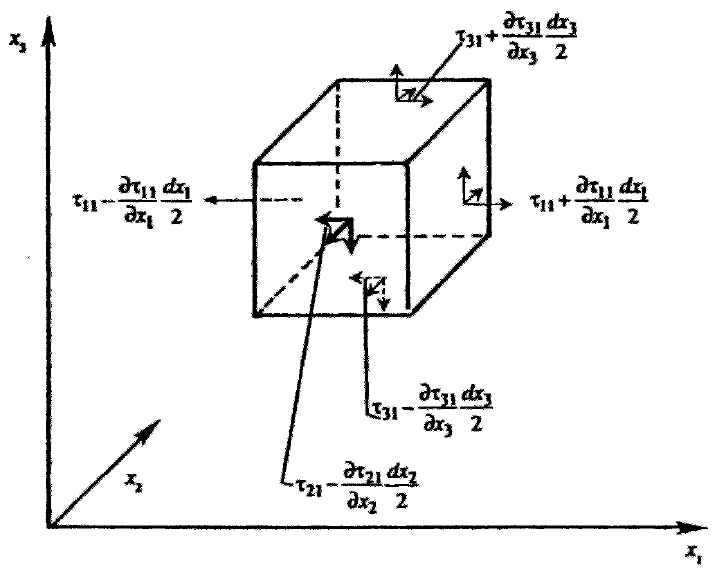
\includegraphics[width=0.5\textwidth,height=0.4\textwidth]{stress.png} 
   \caption{\label{fig:stress} From \cite{kundu2008fluid}.  } 
\end{figure}
%
\end{defn*}




























\subsection{Websites}
\href{http://www2.mpia-hd.mpg.de/homes/dullemon/lectures/hydrodynamicsII/}{Great lecture notes of numerical methods of hydrodynamics}


